\documentclass{beamer}
\usetheme{Copenhagen}
\usepackage{tikz}
\usepackage{multirow}
\usepackage{graphicx}
\usepackage{epstopdf}
\usepackage{subfigure}
\graphicspath{{img/}}

\title[Real-Time Monte Carlo Tree Search in \textit{Ms Pac-Man}]{Real-Time Monte Carlo Tree Search in \textit{Ms Pac-Man}}
\institute{}
\author[Delivered by Chen Shaoyuan]{Original authors: Tom Pepels, Mark H. M. Winands, Marc Lanctot}
\date{December 7, 2017}

\renewcommand{\vec}{\mathbf}
\setlength{\parskip}{0.2cm}

\begin{document}
  \begin{frame}
    \titlepage
  \end{frame}

  \section{Background}
  \begin{frame}{Background}{\textit{Ms Pac-Man}}
    \textit{Ms Pac-Man} is one of \textit{Pac-Man} game series.
    \begin{figure}
      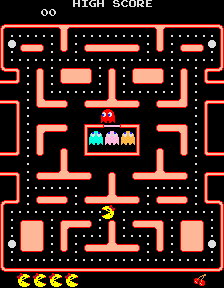
\includegraphics[height = 4.5cm]{mspacman.png}
      \caption{Snapshot of \textit{Ms Pac-Man}}
    \end{figure}
  \end{frame}

  \begin{frame}{Background}{\textit{Ms Pac-Man}}
    \begin{itemize}
      \item Players goal is to avoid being eaten by ghosts and gaining higher scores by collecting pills.
      \item In \textit{Ms Pac-Man}, there are four different mazes, and the behavior of the ghost is unpredictable.
      \item \textit{Ms Pac-Man} has become an interesting topic for AI research.
    \end{itemize}
  \end{frame}

  \section{Monte Carlo Tree Search}
  \begin{frame}{Monte Carlo Tree Search}{Introduction}
  \begin{itemize}
    \item Monte Carlo Tree Search (MCTS) is a best-first search method based on random sampling of the state space for a specified domain.
    \item MCTS has been successfully applied in many turn-based games, such as \textit{Go} and \textit{Hex}.
    \item In MCTS, a tree is built incrementally, and each node keeps statistics corresponding to the reward of that node, and times the nodes have been visited.
    \item MCTS copes well when limited time is available between moves, because it can stop anytime to select a move.
  \end{itemize}
  \end{frame}

  \begin{frame}{Monte Carlo Tree Search}{How it works}
  MCTS consists of four steps, which are performed iteratively.
  \begin{enumerate}
    \item Starting from the root node, choose a child according to some policy, iterating until a leaf node that does not represent a terminal state is reached.
    \item Add children to the selected node given available moves.
    \item Run a simulated playout from the current state randomly, or according to a heuristic strategy, until a terminal is reached.
    \item The result is propagated backward to update the information of the nodes.
  \end{enumerate}
  \end{frame}

  \begin{frame}{Monte Carlo Tree Search}{How it works}
    \begin{figure}
      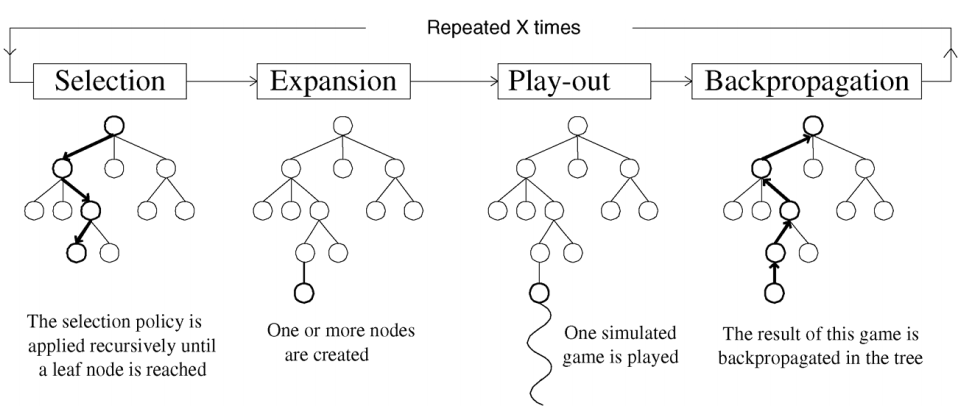
\includegraphics[height = 4.7cm]{mcts_steps.png}
      \caption{Four steps of Mote Carlo tree search}
    \end{figure}
  \end{frame}

  \section{MCTS in Ms Pac-Man}
  \begin{frame}{MCTS in \textit{Ms Pac-Man}}
    Unlike most of the turn-base games, \textit{Ms Pac-Man} is a real-time strategy game. Such games are usually considered more complex than turn based games, including
    \begin{itemize}
      \item The existence of randomness adds uncertainty to the game;
      \item The state space is usually very large;
      \item The game is open-ended.
    \end{itemize}
    \pause
    We would like to apply MCTS framework, but we need to add some enhancements to make it work better.
  \end{frame}

  \begin{frame}{MCTS in \textit{Ms Pac-Man}}{Search Tree and Variable Depth}
    Each node stores reward values for different tactics.

    The cumulative sum of rewards and mean reward are
    \begin{equation} S^{p}_{tactic} = \sum_{n=1}^N R_{tactic,n}^P, \overline{S}^p_{tactic} = \frac{1}{N} \end{equation}

    The maximum mean reward is defined as
    \begin{equation}
      M^p_{tatic} = \begin{cases} \overline{S}^p_{tactic} & \text{if p is a leaf} \\
                                  -\infty & \text{if p is not in the tree} \\
                                  \max_{i \in C(p)} M^i_{tactic} & \text{otherwise}  \end{cases}
    \end{equation}
  \end{frame}

  \begin{frame}{MCTS in \textit{Ms Pac-Man}}{Search Tree and Variable Depth}
    The search path is variably determined by a distance limit $T_{path}$. A leaf is only expanded is the length of the path to the root node does not exceed $T_{path}$.
    \begin{itemize}
      \item this might enable the agent to find safer path when in danger; \par
      \item the scoring potentia over all possible paths in the tree is normalized due to the uniform length of each path.
    \end{itemize}
  \end{frame}

  \begin{frame}{MCTS in \textit{Ms Pac-Man}}{Tactics}
    At any time, one of the following tactics is active:
    \begin{itemize}
      \item If the survival rate is below a threshold, the survival tactic is used;
      \item Otherwise, if a power pill is eaten and edible ghosts are in the range of Pac-Man, the ghost score tactic is selected;
      \item Otherwise, the default pill score tactic is applied.
    \end{itemize}
  \end{frame}

  \begin{frame}{MCTS in \textit{Ms Pac-Man}}{Search tree reuse}
    There are two ways to reuse the tree:
    \begin{description}
      \item[Rule-based reuse] Unless some special situations occur, the search tree is preserved;
      \item[Continuous decay] The values stored in nodes are not discarded, but multiplied by a decay factor $\lambda$. Simulation results suggest that decaying these values $(0 < \lambda < 1)$ can be better compared to no decay $(\lambda = 0)$ and no reuse $(\lambda = 1)$.
    \end{description}
  \end{frame}

  \begin{frame}{MCTS in \textit{Ms Pac-Man}}{Selection and Expansion}
    The policy that determines which child to select is the one that maximized the following equation
    $$ X_i = v_i + C\sqrt{\frac{\ln n_p}{n_i}} $$
    When one or more of the children's visit counts are below a threshold, a random uniform selection is made.
  \end{frame}

  \begin{frame}{MCTS in \textit{Ms Pac-Man}}{Simulation}
    It is neither necessary nor computationally possible to run numerous simulations until the game terminates within strict time limit.

    So, during playout, moves are made until one of the following conditions applies:
    \begin{itemize}
      \item A preset number of time units $T_{time}$ have passed;
      \item Pac-Man is considered dead;
      \item The next maze is reached.
    \end{itemize}
  \end{frame}

  \begin{frame}{MCTS in \textit{Ms Pac-Man}}{Simulation}
    The goals for Pac-Man are
    \begin{itemize}
      \item Keep survived;
      \item Eat more pills;
      \item Eat more ghosts.
    \end{itemize}
    The goals for ghosts are
    \begin{itemize}
      \item Ensure that Pac-Man loses a life by trapping her;
      \item Avoid being eaten by Pac-Man;
      \item Limit the numbers of pills Pac-Man can eat.
    \end{itemize}
  \end{frame}

  \begin{frame}{MCTS in \textit{Ms Pac-Man}}{Backpropagation and move selection}
    \begin{itemize}
      \item If the maximal survival rate is below the threshold, survival tatic should be applied;
      \item Otherwise, scores are determined based on the current tactic;
      \item If the current tactic provides no feasible reward, it is replaced according to the ordering: ghost, pill, survival.
    \end{itemize}
  \end{frame}

  \section{Conclusion}
  \begin{frame}{Conclusion}{Result}
    \begin{figure}
      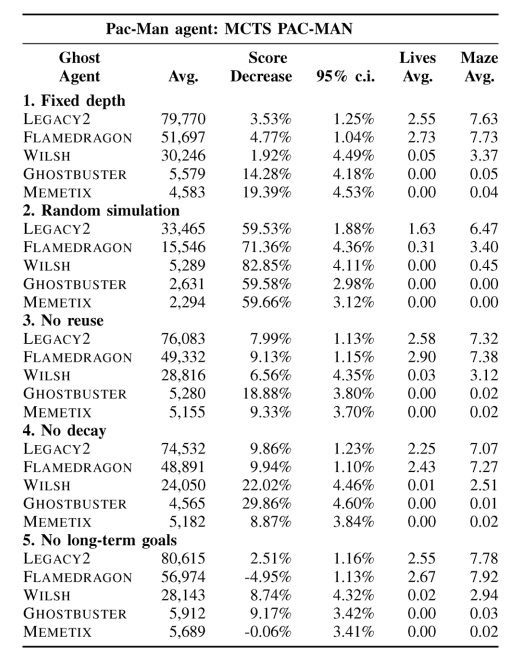
\includegraphics[height = 5cm]{r_single_disabled.png}
      \caption{Single enhancement disabled}
    \end{figure}
  \end{frame}

  \begin{frame}{Conclusion}{Result}
    \begin{figure}
      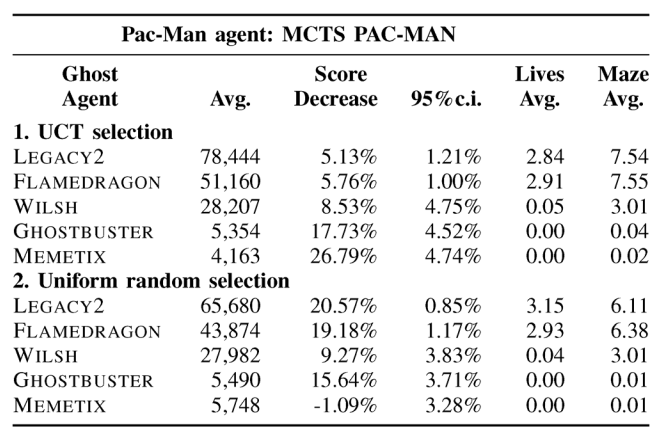
\includegraphics[height = 4.7cm]{r_sim.png}
      \caption{Depth-1 search, simulation strategy}
    \end{figure}
  \end{frame}

  \begin{frame}{Conclusion}{Result}
    \begin{figure}
      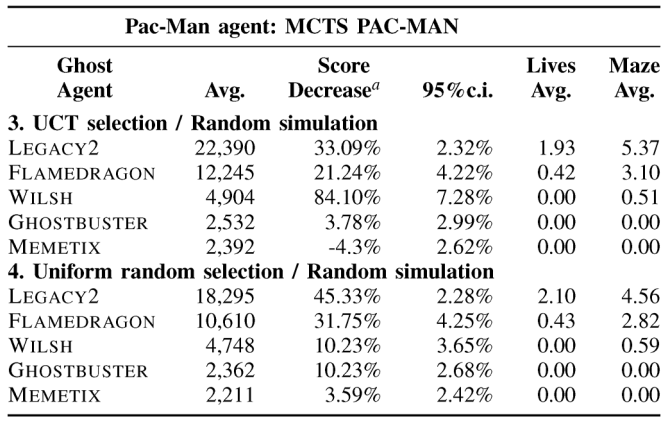
\includegraphics[height = 4.7cm]{r_random.png}
      \caption{Depth-1 search, random simulation}
    \end{figure}
  \end{frame}

  \section{}
  \begin{frame}{Q \& A}

  \end{frame}
\end{document}
